% Block diagram of bnn_top for P = 1.
% Build (from docs/):  pdflatex -output-directory=../build/latex block_diagram_p1.tex
% Plain article class (no standalone.cls needed); the PDF page is sized to the
% diagram at the end of the file.
\documentclass{article}
\usepackage{tikz}
\usetikzlibrary{positioning,arrows.meta,calc}
\pagestyle{empty}
\newsavebox{\diagram}

\tikzset{
  >={Stealth[length=2.2mm]},
  every node/.style={font=\small},
  ff/.style  ={draw,thick,fill=blue!7,minimum width=11mm,minimum height=8mm,inner sep=0pt},
  rom/.style ={draw,thick,fill=orange!12,minimum height=10mm,minimum width=18mm,align=center},
  comb/.style={draw,thick,fill=green!9,rounded corners=3pt,minimum height=16mm,minimum width=30mm,align=center},
  blk/.style ={draw,thick,rounded corners=2pt,minimum height=12mm,align=center},
  ctrl/.style={draw,thick,fill=red!6,rounded corners=2pt,minimum height=16mm,align=center},
  region/.style={draw=gray!60,dashed,rounded corners=4pt},
  rlabel/.style={font=\small\bfseries,text=gray!80!black},
  sig/.style ={font=\scriptsize\itshape,text=red!65!black},   % control signal name
  w/.style   ={font=\scriptsize,midway,above},                % bus width / net name
  pin/.style ={font=\tiny,inner sep=1pt},
  bus/.style ={->,thick},
  dot/.style ={circle,fill,inner sep=1.3pt},
}

% Flip-flop pin labels: D (upper left), EN (lower left), Q (right) and the
% clock triangle on the bottom edge. #2 = horizontal offset of the triangle.
\newcommand{\ffpins}[2]{%
  \node[pin,anchor=west] at ([yshift=2mm]#1.west)  {D};
  \node[pin,anchor=west] at ([yshift=-2mm]#1.west) {EN};
  \node[pin,anchor=east] at (#1.east) {Q};
  \draw[thin] ([xshift=#2-1.2mm]#1.south) -- ([xshift=#2,yshift=1.4mm]#1.south)
              -- ([xshift=#2+1.2mm]#1.south);}

\begin{document}
\begin{lrbox}{\diagram}
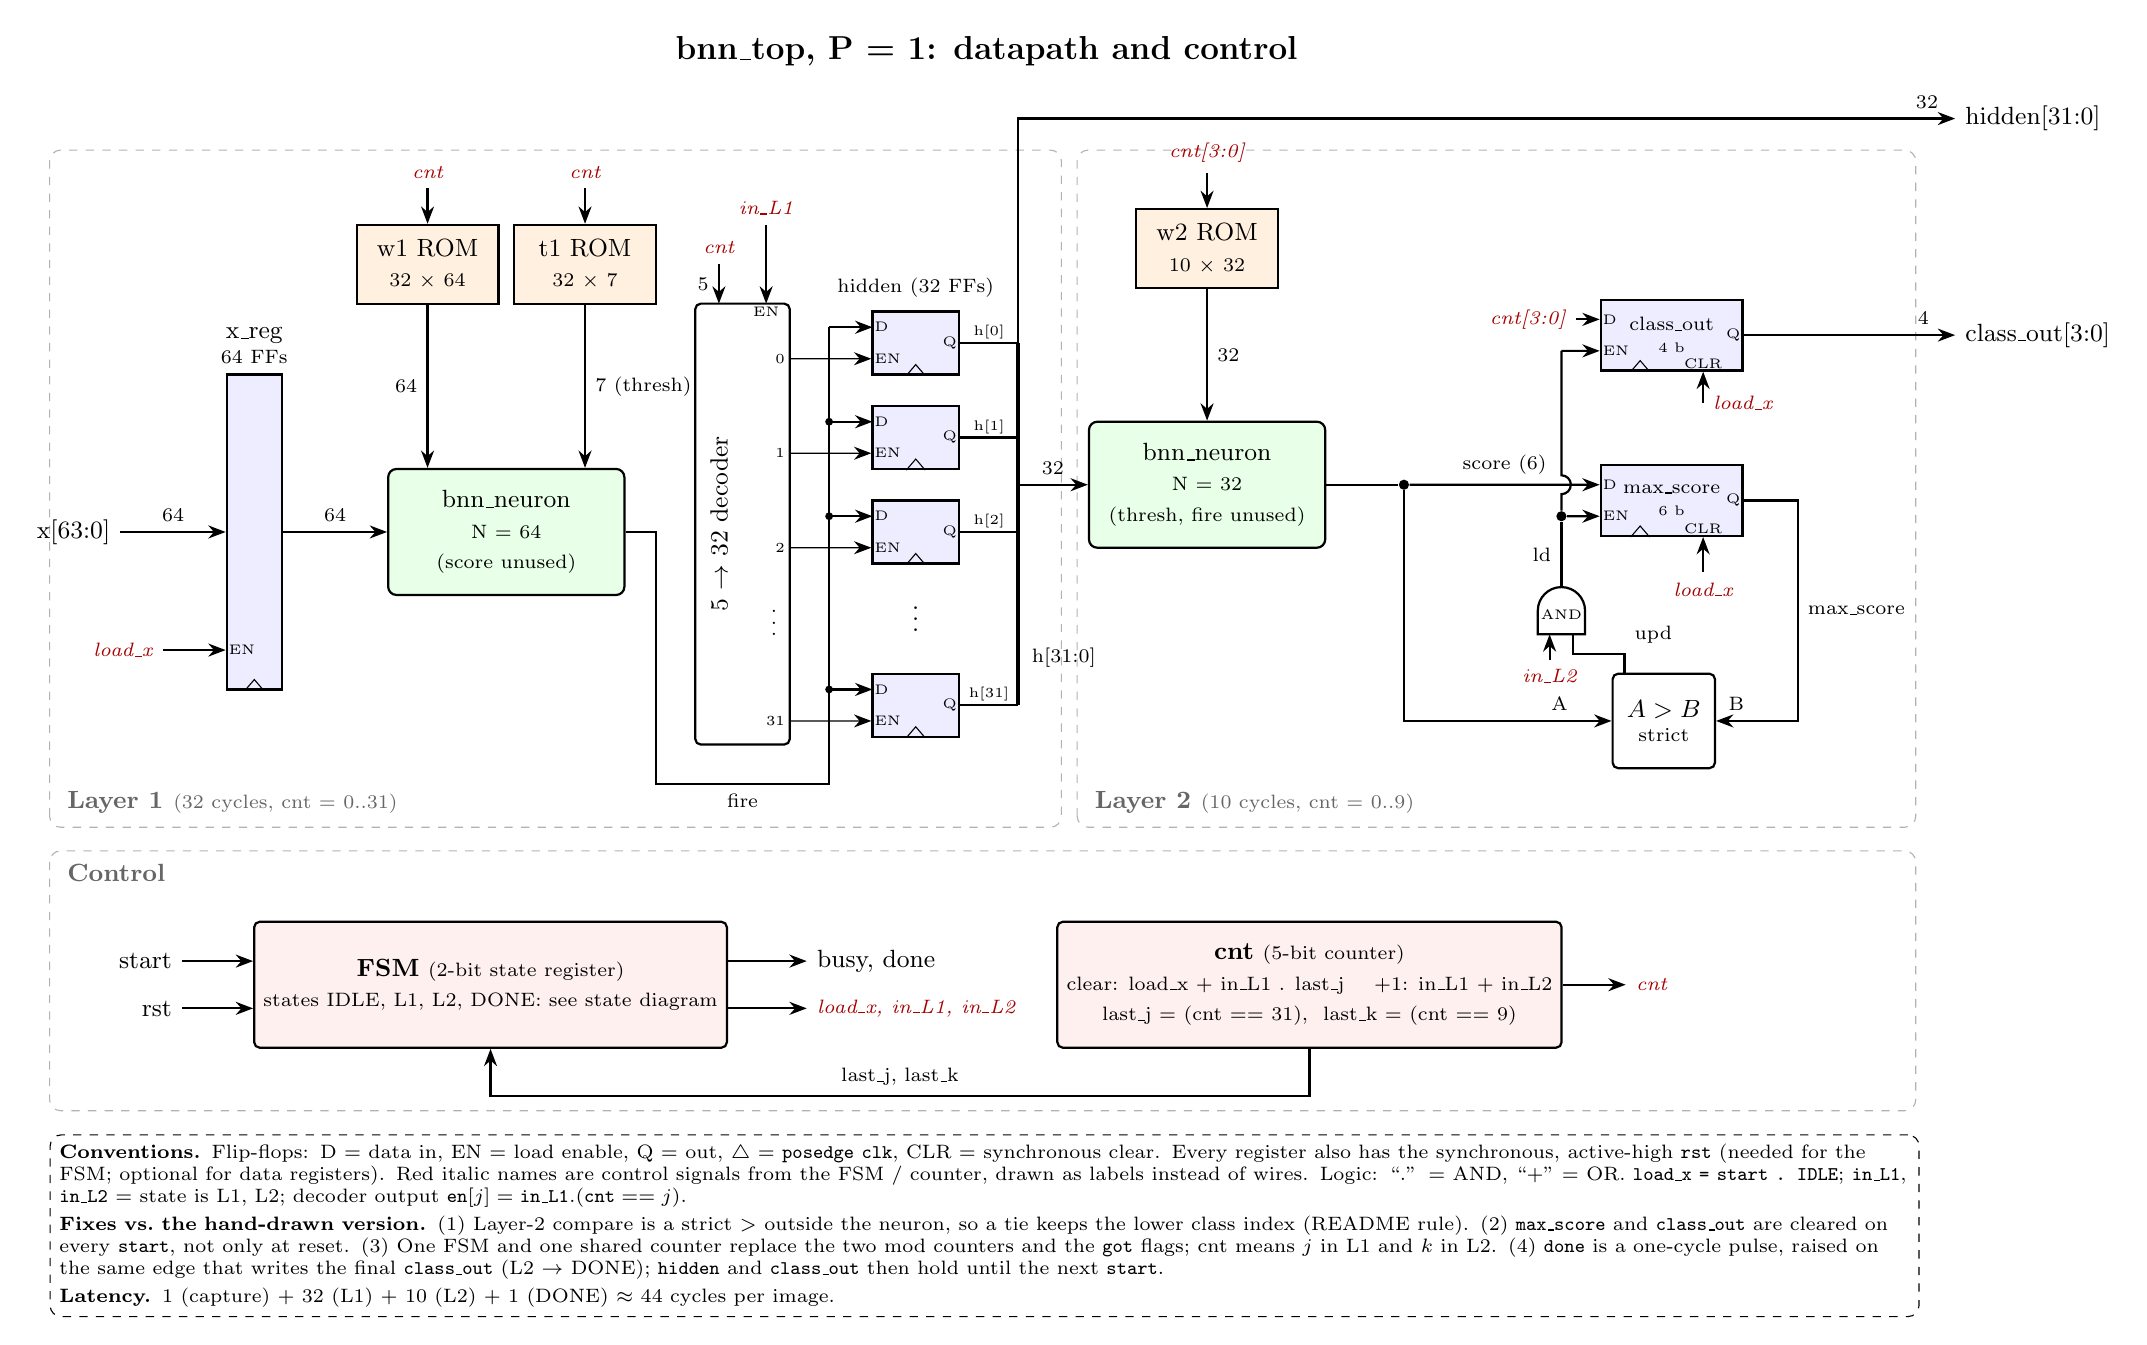
\begin{tikzpicture}

\node[font=\large\bfseries] at (9.3,6.1) {bnn\_top, P = 1: datapath and control};

% ---------------------------------------------------------------- regions
\draw[region] (-2.6,-3.75) rectangle (10.25,4.85);
\node[rlabel,anchor=south west] at (-2.5,-3.7) {Layer 1 \textmd{\scriptsize (32 cycles, cnt = 0..31)}};
\draw[region] (10.45,-3.75) rectangle (21.1,4.85);
\node[rlabel,anchor=south west] at (10.55,-3.7) {Layer 2 \textmd{\scriptsize (10 cycles, cnt = 0..9)}};
\draw[region] (-2.6,-4.05) rectangle (21.1,-7.35);
\node[rlabel,anchor=north west] at (-2.5,-4.1) {Control};

% ================================================================ LAYER 1
% x_reg: 64-bit pipeline-style register bar
\node[draw,thick,fill=blue!7,minimum width=7mm,minimum height=40mm,inner sep=0pt,
      label={[align=center]above:{x\_reg\\[-2pt]\scriptsize 64 FFs}}] (xreg) at (0,0) {};
\draw[thin] ([xshift=-1.2mm]xreg.south) -- ([yshift=1.4mm]xreg.south) -- ([xshift=1.2mm]xreg.south);
\node[pin,anchor=west] at ([yshift=-15mm]xreg.west) {EN};
\draw[bus] (-1.7,0) node[left]{x[63:0]} -- node[w]{64} (xreg.west);
\draw[<-,thick] ([yshift=-15mm]xreg.west) -- ++(-0.8,0) node[left,sig]{load\_x};

% layer-1 neuron and its ROMs
\node[comb] (n1) at (3.2,0) {bnn\_neuron\\\scriptsize N = 64\\\scriptsize (score unused)};
\draw[bus] (xreg.east) -- node[w]{64} (n1.west);
\node[rom] (w1) at (2.2,3.4) {w1 ROM\\\scriptsize 32 $\times$ 64};
\node[rom] (t1) at (4.2,3.4) {t1 ROM\\\scriptsize 32 $\times$ 7};
\draw[bus] (w1.south) -- node[left,font=\scriptsize]{64} (w1.south |- n1.north);
\draw[bus] (t1.south) -- node[right,font=\scriptsize]{7 (thresh)} (t1.south |- n1.north);
\draw[<-,thick] (w1.north) -- ++(0,0.45) node[above,sig]{cnt};
\draw[<-,thick] (t1.north) -- ++(0,0.45) node[above,sig]{cnt};

% 5 -> 32 decoder (vertical)
\draw[thick,fill=white,rounded corners=2pt] (5.6,-2.7) rectangle (6.8,2.9);
\node[rotate=90] at (5.9,0.1) {5 $\to$ 32 decoder};
\draw[<-,thick] (5.9,2.9) -- node[left,font=\scriptsize]{5} (5.9,3.4) node[above,sig]{cnt};
\node[pin,anchor=north] at (6.5,2.9) {EN};
\draw[<-,thick] (6.5,2.9) -- (6.5,3.9) node[above,sig]{in\_L1};

% hidden register: 32 individual FFs (h[0], h[1], h[2], ..., h[31])
\foreach \n/\y/\lbl/\idx in {h0/2.4/h[0]/0, h1/1.2/h[1]/1, h2/0.0/h[2]/2, h31/-2.2/h[31]/31} {
  \node[ff] (\n) at (8.4,\y) {};
  \ffpins{\n}{0mm}
  % enable from the decoder
  \draw[->,thin] (6.8,\y-0.2) -- ([yshift=-2mm]\n.west);
  \node[pin,anchor=east] at (6.78,\y-0.2) {\idx};
  % Q into the merge bus
  \draw[thick] (\n.east) -- node[above,pin]{\lbl} (9.7,\y);
}
\node at (8.4,-1.0) {$\vdots$};
\node at (6.6,-1.05) {\scriptsize$\vdots$};
\node[font=\scriptsize,anchor=south] at (8.4,2.85) {hidden (32 FFs)};

% fire: one line to every D input
\draw[thick] (n1.east) -- (5.1,0) -- (5.1,-3.2) -- node[below,font=\scriptsize]{fire} (7.3,-3.2) -- (7.3,2.6);
\foreach \y in {1.2, 0.0, -2.2} {
  \node[dot,inner sep=1pt] at (7.3,\y+0.2) {};
  \draw[->,thick] (7.3,\y+0.2) -- (8.4-0.55,\y+0.2);
}
\draw[->,thick] (7.3,2.6) -- (8.4-0.55,2.6);

% merge bus h[31:0]
\draw[line width=1.6pt] (9.7,2.4) -- (9.7,-2.2);
\node[font=\scriptsize,anchor=west] at (9.75,-1.6) {h[31:0]};

% hidden -> output port (along the top)
\draw[bus] (9.7,2.4) -- (9.7,5.25) -- node[w,pos=0.97]{32} (21.6,5.25) node[right]{hidden[31:0]};

% ================================================================ LAYER 2
\node[comb] (n2) at (12.1,0.6) {bnn\_neuron\\\scriptsize N = 32\\\scriptsize (thresh, fire unused)};
\draw[bus] (9.7,0.6) -- node[w]{32} (n2.west);
\node[rom] (w2) at (12.1,3.6) {w2 ROM\\\scriptsize 10 $\times$ 32};
\draw[bus] (w2.south) -- node[right,font=\scriptsize]{32} (n2.north);
\draw[<-,thick] (w2.north) -- ++(0,0.45) node[above,sig]{cnt[3:0]};

% Two separate registers, both loaded by ld = in_L2 . upd (wired).
% class_out sits above max_score so the max_score feedback never crosses an output.
\node[dot] (sb) at (14.6,0.6) {};
\draw[thick] (n2.east) -- (sb);

% max_score FF (on the score row)
\node[ff,minimum width=18mm,minimum height=9mm,align=center] (mreg) at (18.0,0.4)
     {\scriptsize max\_score\\[-3pt]\tiny 6 b};
\ffpins{mreg}{-4mm}
\node[pin,anchor=south] at ([xshift=4mm]mreg.south) {CLR};
\draw[bus] (sb) -- node[w]{score (6)} ([yshift=2mm]mreg.west);
\draw[<-,thick] ([xshift=4mm]mreg.south) -- ++(0,-0.45) node[below,sig]{load\_x};

% class_out FF (above)
\node[ff,minimum width=18mm,minimum height=9mm,align=center] (creg) at (18.0,2.5)
     {\scriptsize class\_out\\[-3pt]\tiny 4 b};
\ffpins{creg}{-4mm}
\node[pin,anchor=south] at ([xshift=4mm]creg.south) {CLR};
\draw[<-,thick] ([yshift=2mm]creg.west) -- ++(-0.3,0) node[left,sig]{cnt[3:0]};
\draw[<-,thick] ([xshift=4mm]creg.south) -- ++(0,-0.4) node[right,sig]{load\_x};
\draw[bus] (creg.east) -- node[w,pos=0.85]{4} (21.6,2.5) node[right]{class\_out[3:0]};

% strict comparator: A = new score, B = max_score so far
\node[blk,minimum width=13mm] (cmp) at (17.9,-2.4) {$A > B$\\[-2pt]\scriptsize strict};
\draw[bus] (sb) -- (14.6,-2.4) -- node[above,font=\scriptsize,pos=0.75]{A} (cmp.west);
\draw[bus] (mreg.east) -- (19.6,0.4) -- node[right,font=\scriptsize]{max\_score} (19.6,-2.4)
           -- node[above,font=\scriptsize,pos=0.75]{B} (cmp.east);

% AND gate (pointing up): ld = in_L2 . upd, wired to both EN pins
\draw[thick,fill=white] (16.3,-1.3) -- (16.3,-1.0) arc[start angle=180,end angle=0,radius=0.3]
                        -- (16.9,-1.3) -- cycle;
\node[font=\tiny] at (16.6,-1.05) {AND};
\draw[thick] (17.4,-1.8) -- (17.4,-1.55) -- node[above,font=\scriptsize,pos=0.0,anchor=south west]{upd} (16.75,-1.55)
             -- (16.75,-1.3);
\draw[<-,thick] (16.45,-1.3) -- (16.45,-1.62) node[below,sig]{in\_L2};
\node[dot] (ldd) at (16.6,0.2) {};
\draw[thick] (16.6,-0.7) -- node[left,font=\scriptsize]{ld} (ldd);
\draw[->,thick] (ldd) -- ([yshift=-2mm]mreg.west);
% ld continues up to class_out EN, hopping over the score line
\draw[thick] (ldd) -- (16.6,0.48) arc[start angle=-90,end angle=90,radius=0.12] -- (16.6,2.3);
\draw[->,thick] (16.6,2.3) -- ([yshift=-2mm]creg.west);

% ================================================================ CONTROL
\node[ctrl,minimum width=46mm] (fsm) at (3.0,-5.75)
     {\textbf{FSM} {\scriptsize (2-bit state register)}\\
      \scriptsize states IDLE, L1, L2, DONE: see state diagram};
\draw[<-,thick] ([yshift=3mm]fsm.west)  -- ++(-0.9,0) node[left]{start};
\draw[<-,thick] ([yshift=-3mm]fsm.west) -- ++(-0.9,0) node[left]{rst};
\draw[bus] ([yshift=3mm]fsm.east)  -- ++(1.0,0) node[right]{busy, done};
\draw[bus] ([yshift=-3mm]fsm.east) -- ++(1.0,0) node[right,sig]{load\_x, in\_L1, in\_L2};

\node[ctrl,minimum width=46mm] (cnt) at (13.4,-5.75)
     {\textbf{cnt} {\scriptsize (5-bit counter)}\\
      \scriptsize clear: load\_x + in\_L1 . last\_j \quad +1: in\_L1 + in\_L2\\
      \scriptsize last\_j = (cnt == 31), \ last\_k = (cnt == 9)};
\draw[bus] (cnt.east) -- ++(0.8,0) node[right,sig]{cnt};
\draw[bus] (cnt.south) -- ++(0,-0.6) -| node[pos=0.25,above,font=\scriptsize]{last\_j, last\_k} (fsm.south);

% ================================================================ NOTES
\node[draw,dashed,rounded corners,anchor=north west,text width=23.5cm,align=left,font=\scriptsize]
     at (-2.6,-7.65) {%
  \textbf{Conventions.} Flip-flops: D = data in, EN = load enable, Q = out, $\triangle$ = \texttt{posedge clk},
  CLR = synchronous clear. Every register also has the synchronous, active-high \texttt{rst} (needed for the FSM;
  optional for data registers). Red italic names are control signals from the FSM / counter, drawn as labels instead
  of wires. Logic: ``.'' = AND, ``+'' = OR.
  \texttt{load\_x = start . IDLE};\ \texttt{in\_L1}, \texttt{in\_L2} = state is L1, L2;\
  decoder output $\mathtt{en}[j] = \mathtt{in\_L1} . (\mathtt{cnt} == j)$.\\[2pt]
  \textbf{Fixes vs.\ the hand-drawn version.}
  (1) Layer-2 compare is a strict $>$ outside the neuron, so a tie keeps the lower class index (README rule).
  (2) \texttt{max\_score} and \texttt{class\_out} are cleared on every \texttt{start}, not only at reset.
  (3) One FSM and one shared counter replace the two mod counters and the \texttt{got} flags; cnt means $j$ in L1
      and $k$ in L2.
  (4) \texttt{done} is a one-cycle pulse, raised on the same edge that writes the final \texttt{class\_out}
      (L2 $\to$ DONE); \texttt{hidden} and \texttt{class\_out} then hold until the next \texttt{start}.\\[2pt]
  \textbf{Latency.} 1 (capture) + 32 (L1) + 10 (L2) + 1 (DONE) $\approx$ 44 cycles per image.
};

\end{tikzpicture}
\end{lrbox}

% Size the PDF page to the diagram plus a 1 cm margin (pdflatex).
\pdfpagewidth=\dimexpr\wd\diagram+2cm\relax
\pdfpageheight=\dimexpr\ht\diagram+\dp\diagram+2cm\relax
\hoffset=-1in \voffset=-1in
\oddsidemargin=1cm \topmargin=1cm \headheight=0pt \headsep=0pt \topskip=0pt
\textwidth=\wd\diagram \hsize=\textwidth
\textheight=\dimexpr\ht\diagram+\dp\diagram+1pt\relax \vsize=\textheight
\noindent\usebox{\diagram}
\end{document}
